% Use with CC terms.
% Adrin Jalali - 2013
%

\documentclass[final]{beamer} % beamer 3.10: do NOT use option hyperref={pdfpagelabels=false} !
%\documentclass[final,hyperref={pdfpagelabels=false}]{beamer} % beamer 3.07: get rid of beamer warnings
\mode<presentation> {  %% check http://www-i6.informatik.rwth-aachen.de/~dreuw/latexbeamerposter.php for examples
  \usetheme{Berlin}  
}
\usepackage[english]{babel}
\usepackage[latin1]{inputenc}
\usepackage{amsmath,amsthm, amssymb, latexsym}
\usefonttheme[onlymath]{serif}
\boldmath
\usepackage[size=custom,width=95,height=130,scale=2,debug]{beamerposter}


\usepackage{beamerthemeshadow}
\usepackage[absolute,overlay]{textpos}
\usepackage{graphics}
\usepackage{colortbl}
\usepackage{xcolor}
\usepackage[absolute,overlay]{textpos}
\usepackage{sidecap}
\usepackage[labelformat=empty]{caption}
\usepackage{booktabs}

\setbeamercolor{framesource}{fg=gray}
\setbeamerfont{framesource}{size=\tiny}
\beamertemplatenavigationsymbolsempty

\newcommand{\source}[1]{\begin{textblock*}{4cm}(8.7cm,8.6cm)
    \begin{beamercolorbox}[ht=0.5cm,right]{framesource}
        \usebeamerfont{framesource}\usebeamercolor[fg]{framesource} {#1}
    \end{beamercolorbox}
\end{textblock*}}

\newcommand{\mycite}[1]{\begin{textblock*}{4cm}(8.7cm,8.6cm)
    \begin{beamercolorbox}[ht=0.5cm,right]{framesource}
        \usebeamerfont{framesource}\usebeamercolor[fg]{framesource} {#1}
    \end{beamercolorbox}
\end{textblock*}}

\definecolor{pathwaynode}{RGB}{255,150,50}
\definecolor{independentnode}{RGB}{255,255,50}
\newcommand{\boz}{\cellcolor{pathwaynode}}
\newcommand{\ghool}{\cellcolor{independentnode}}

\title[Gene Expression, PPI Network, Classification]{Analyzing How Protein Interaction Networks Improve Classification Performance in Gene Expression Data Analysis}
\author[Adrin Jalali]{Adrin Jalali \\ \small{Supervised by: Nico Pfeifer}}
\institute{MPI for Informatics}
\date{\today} 
\titlegraphic{
\includegraphics[width=4cm]{mpi-logo}}
\begin{document}
\begin{frame}{} 
  \maketitle
  \begin{block}{Data}
    \begin{columns}[T]
      \begin{column}{0.3\textwidth}
        \begin{columns}
          \begin{column}{0.5\textwidth}
            \begin{figure}
              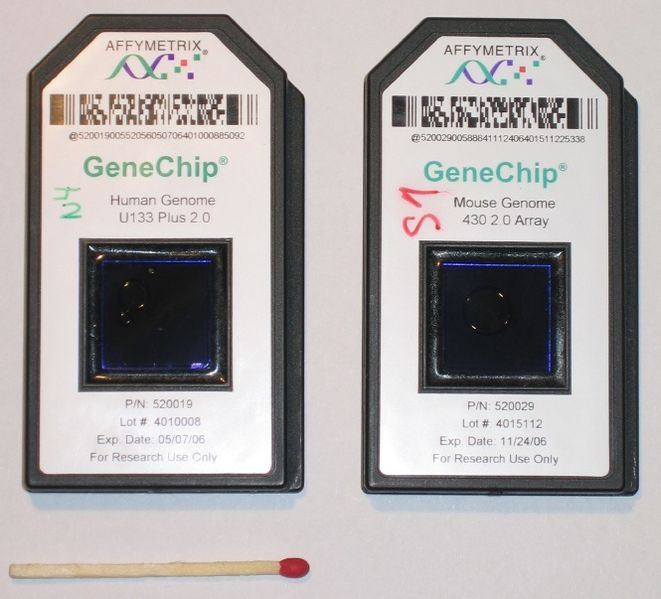
\includegraphics[width=0.9\textwidth]{Affymetrix-microarray}
            \end{figure}
          \end{column}
          \begin{column}{0.5\textwidth}
            \begin{figure}
              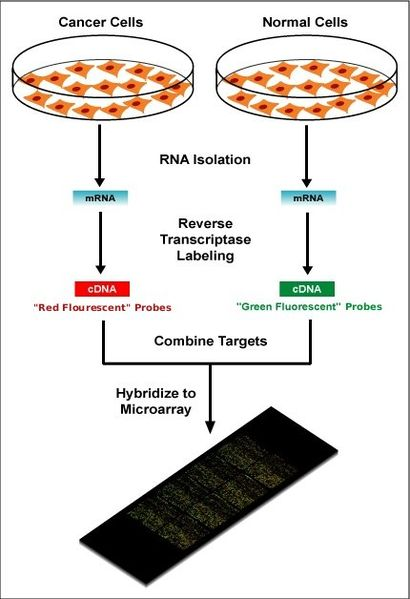
\includegraphics[width=0.8\textwidth]{Microarray-schema}
              \caption{\tiny Microarray Gene Expression Data}
            \end{figure}
          \end{column}
        \end{columns}
        %\source{en.wikipedia.org}
        \note{http://en.wikipedia.org/wiki/DNA_microarray}
      \end{column}

      \begin{column}{0.25\textwidth}
        \center
        \begin{figure}
          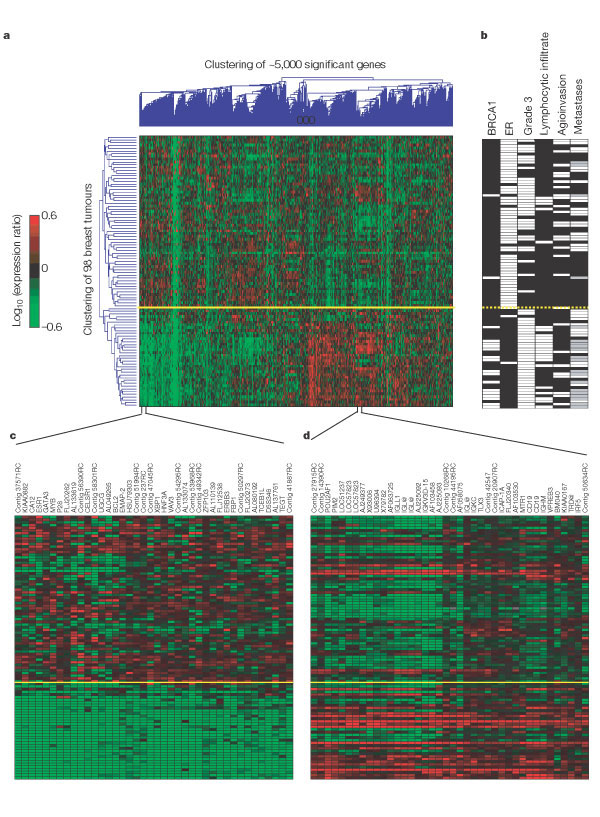
\includegraphics[width=0.7\textwidth]{vantveer-summary}
          \caption{\tiny
            1. Input: Gene expression data
            2. Output: Prognosis (Poor vs. Good), Metastases
            3. Goal: Classify and find important genes
            4. Issue: Hard to classify due to huge number of features (genes) compared to number of samples ($\sim 22000 \gg 98$)\\
            - Laura J. van 't Veer et.al. Nature, (2002)}
          \note{a, Two-dimensional presentation of transcript ratios for 98 breast tumours. There were 4,968 significant genes across the group. Each row represents a tumour and each column a single gene. As shown in the colour bar, red indicates upregulation, green downregulation, black no change, and grey no data available. The yellow line marks the subdivision into two dominant tumour clusters. b, Selected clinical data for the 98 patients in a: BRCA1 germline mutation carrier (or sporadic patient), ER expression, tumour grade 3 (versus grade 1 and 2), lymphocytic infiltrate, angioinvasion, and metastasis status. White indicates positive, black negative and grey denotes tumours derived from BRCA1 germline carriers who were excluded from the metastasis evaluation. The cluster below the yellow line consists of 36 tumours, of which 34 are ER negative (total 39 ER-negative) and 16 are carriers of the BRCA1 mutation (total 18). c, Enlarged portion from a containing a group of genes that co-regulate with the ER- gene (ESR1). Each gene is labelled by its gene name or accession number from GenBank. Contig ESTs ending with RC are reverse-complementary of the named contig EST. d, Enlarged portion from a containing a group of co-regulated genes that are the molecular reflection of extensive lymphocytic infiltrate, and comprise a set of genes expressed in T and B cells. (Gene annotation as in c.)}
          \note{http://www.nature.com/nature/journal/v415/n6871/full/415530a.html}
        \end{figure}
      \end{column}

      \begin{column}{0.25\paperwidth}
        \begin{figure}
          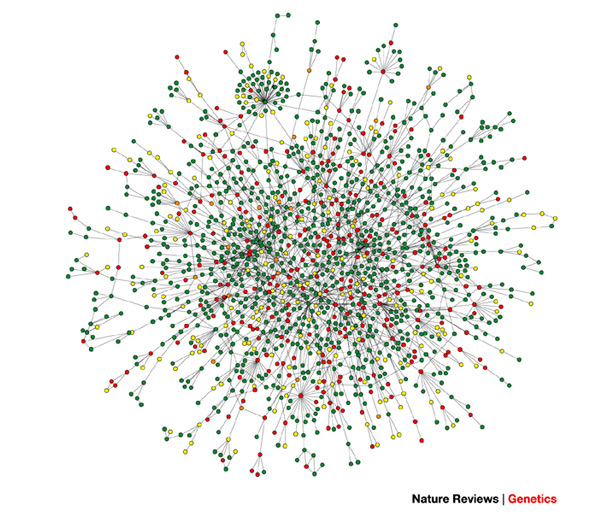
\includegraphics[width=0.6\textwidth]{yeastProteinInteractionNetwork}
          \caption{\tiny Yeast protein interaction network. The colour of a node indicates the phenotypic effect of removing the corresponding protein ({\color{red}red} = lethal, {\color{green}green} = non-lethal, {\color{orange}orange} = slow growth, {\color{yellow}yellow} = unknown), A. Barabási, Z. Oltvai, Nature Reviews Genetics, (2004)}
        \end{figure}
        \note{http://www.nature.com/nrg/journal/v5/n2/fig_tab/nrg1272_F2.html}
      \end{column}
      \begin{column}{0.3\textwidth}
        %\frametitle{NICK Performance Summary}
        \begin{figure}
          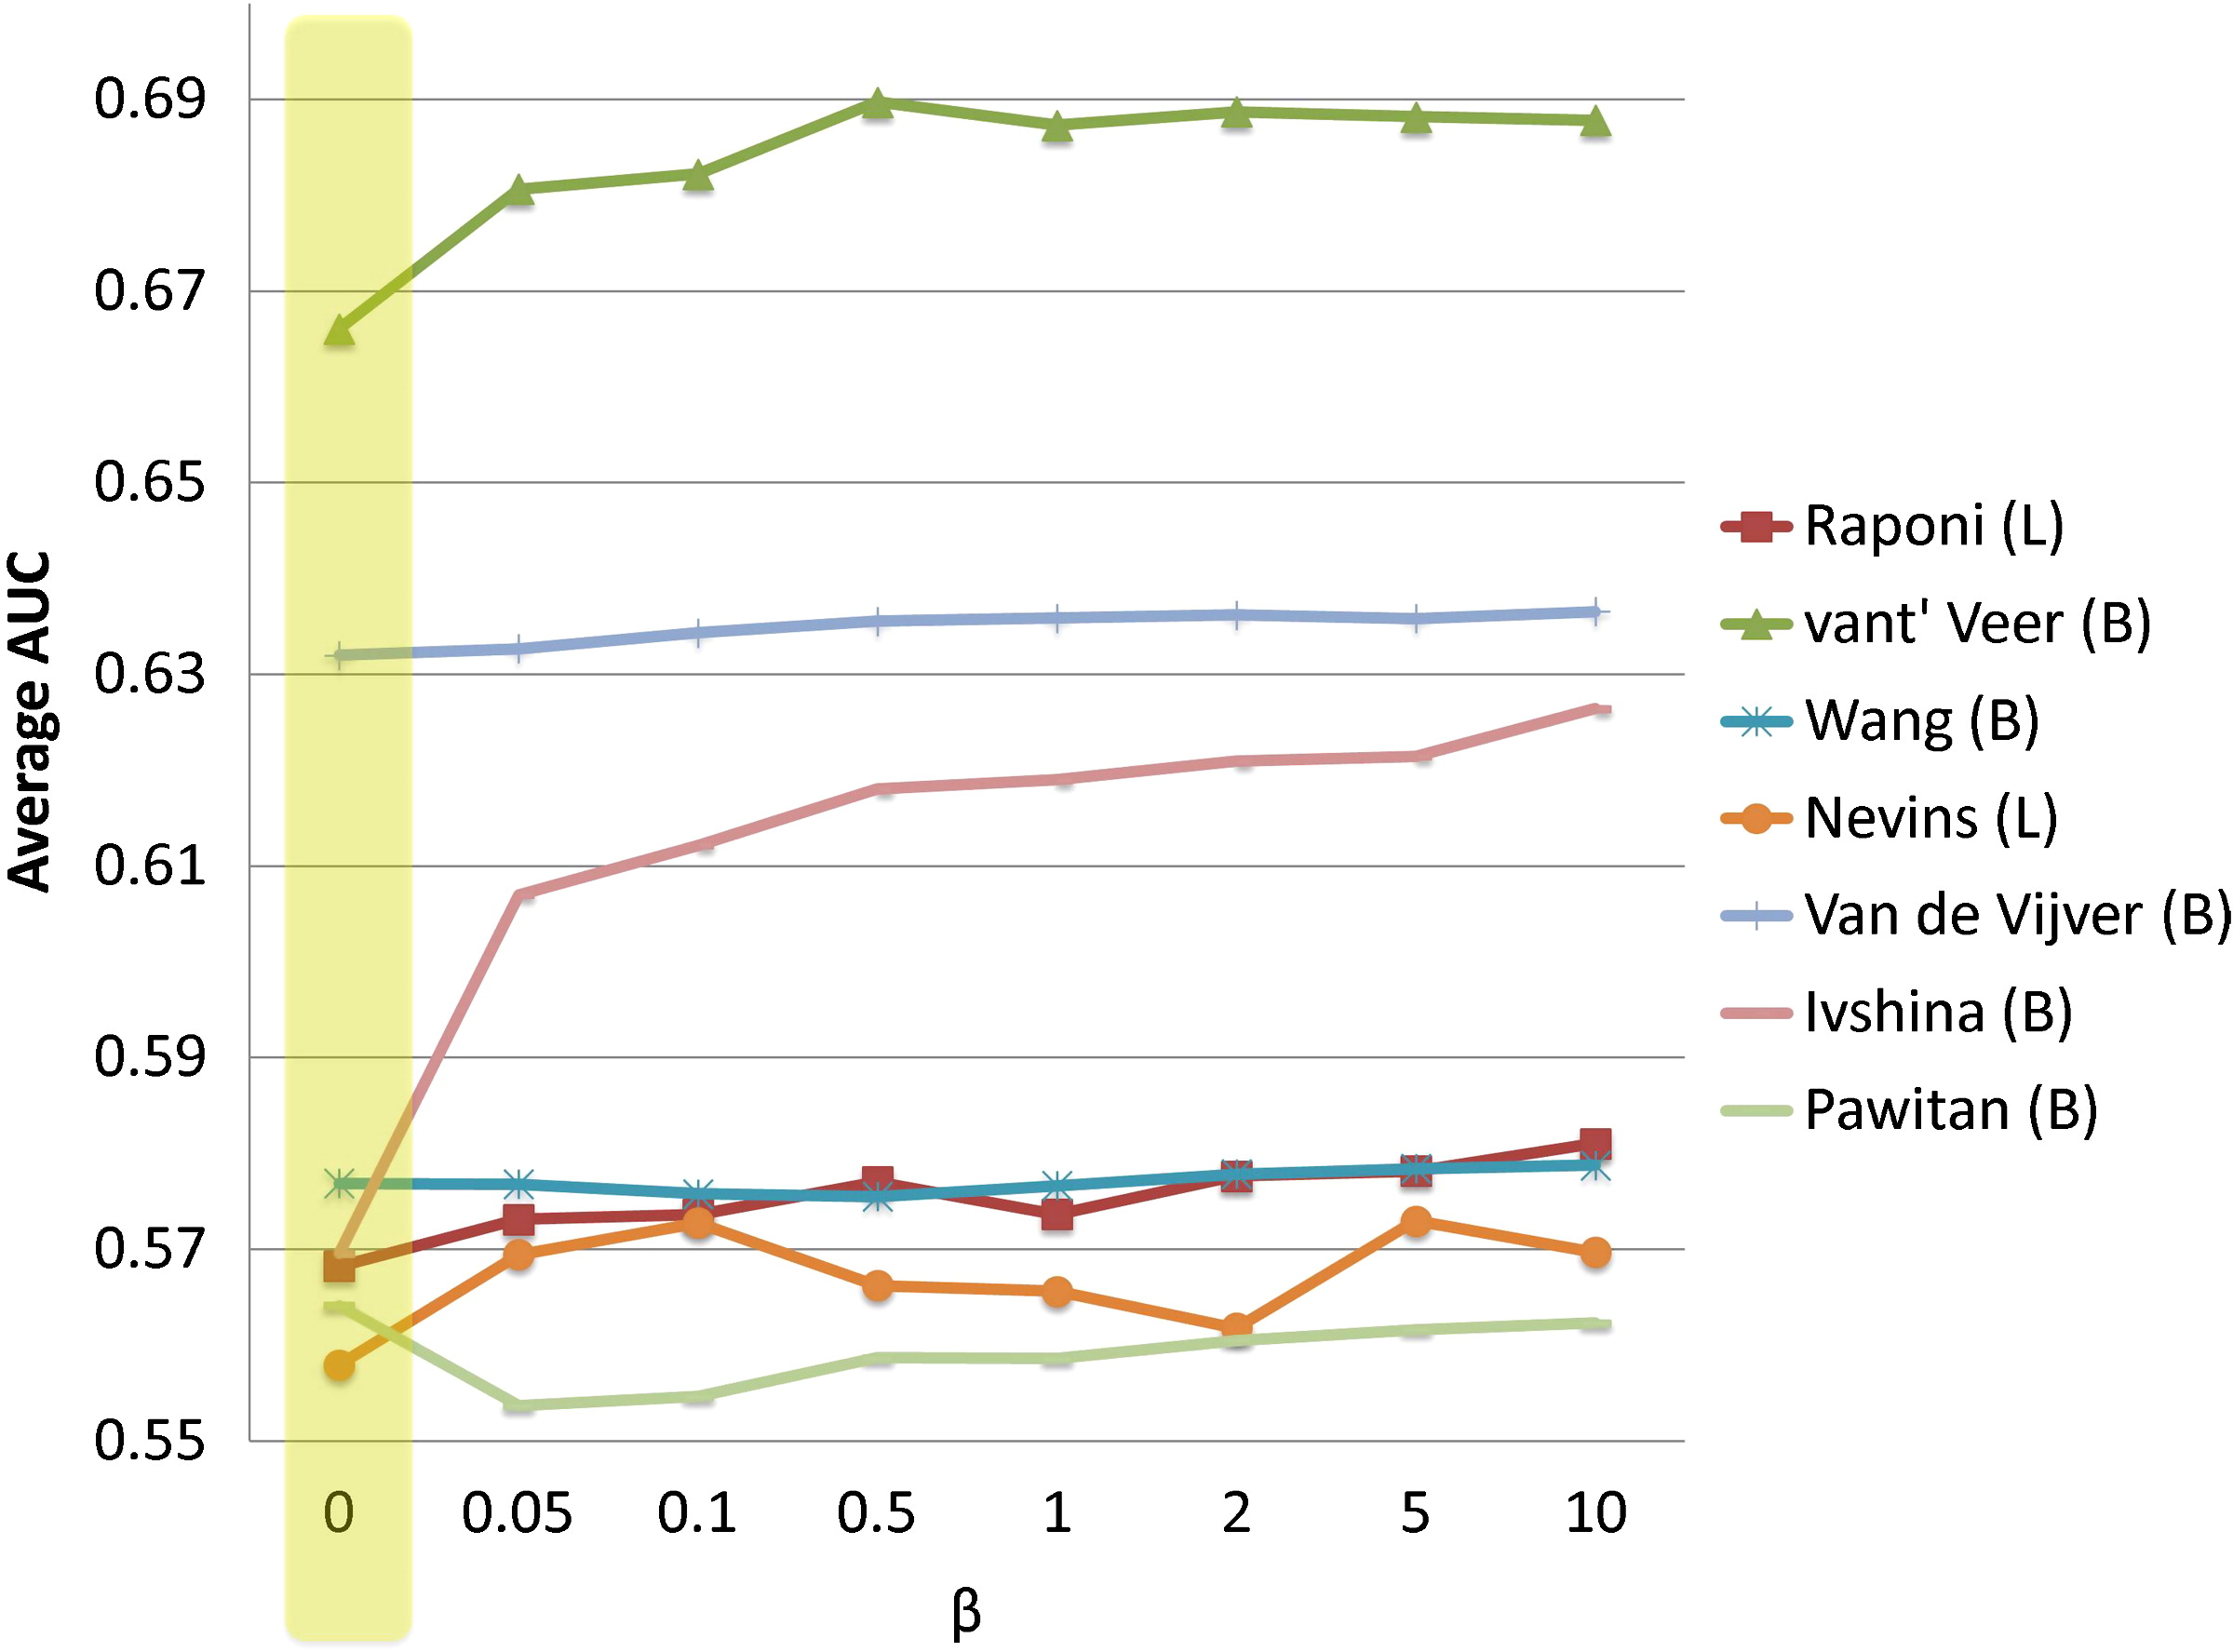
\includegraphics[width=0.8\textwidth]{NICK-perfs}
        \end{figure}
        %\mycite{Ofer Lavi, et.al., Journal of Computational Biology, (2012)}
        \note{http://online.liebertpub.com/doi/full/10.1089/cmb.2012.0065}
      \end{column}
    \end{columns}
  \end{block}

  \begin{block}{Method}
    \begin{columns}
      \begin{column}{0.3\textwidth}
        \begin{columns}
          \begin{column}{0.5\textwidth}
            \begin{figure}
              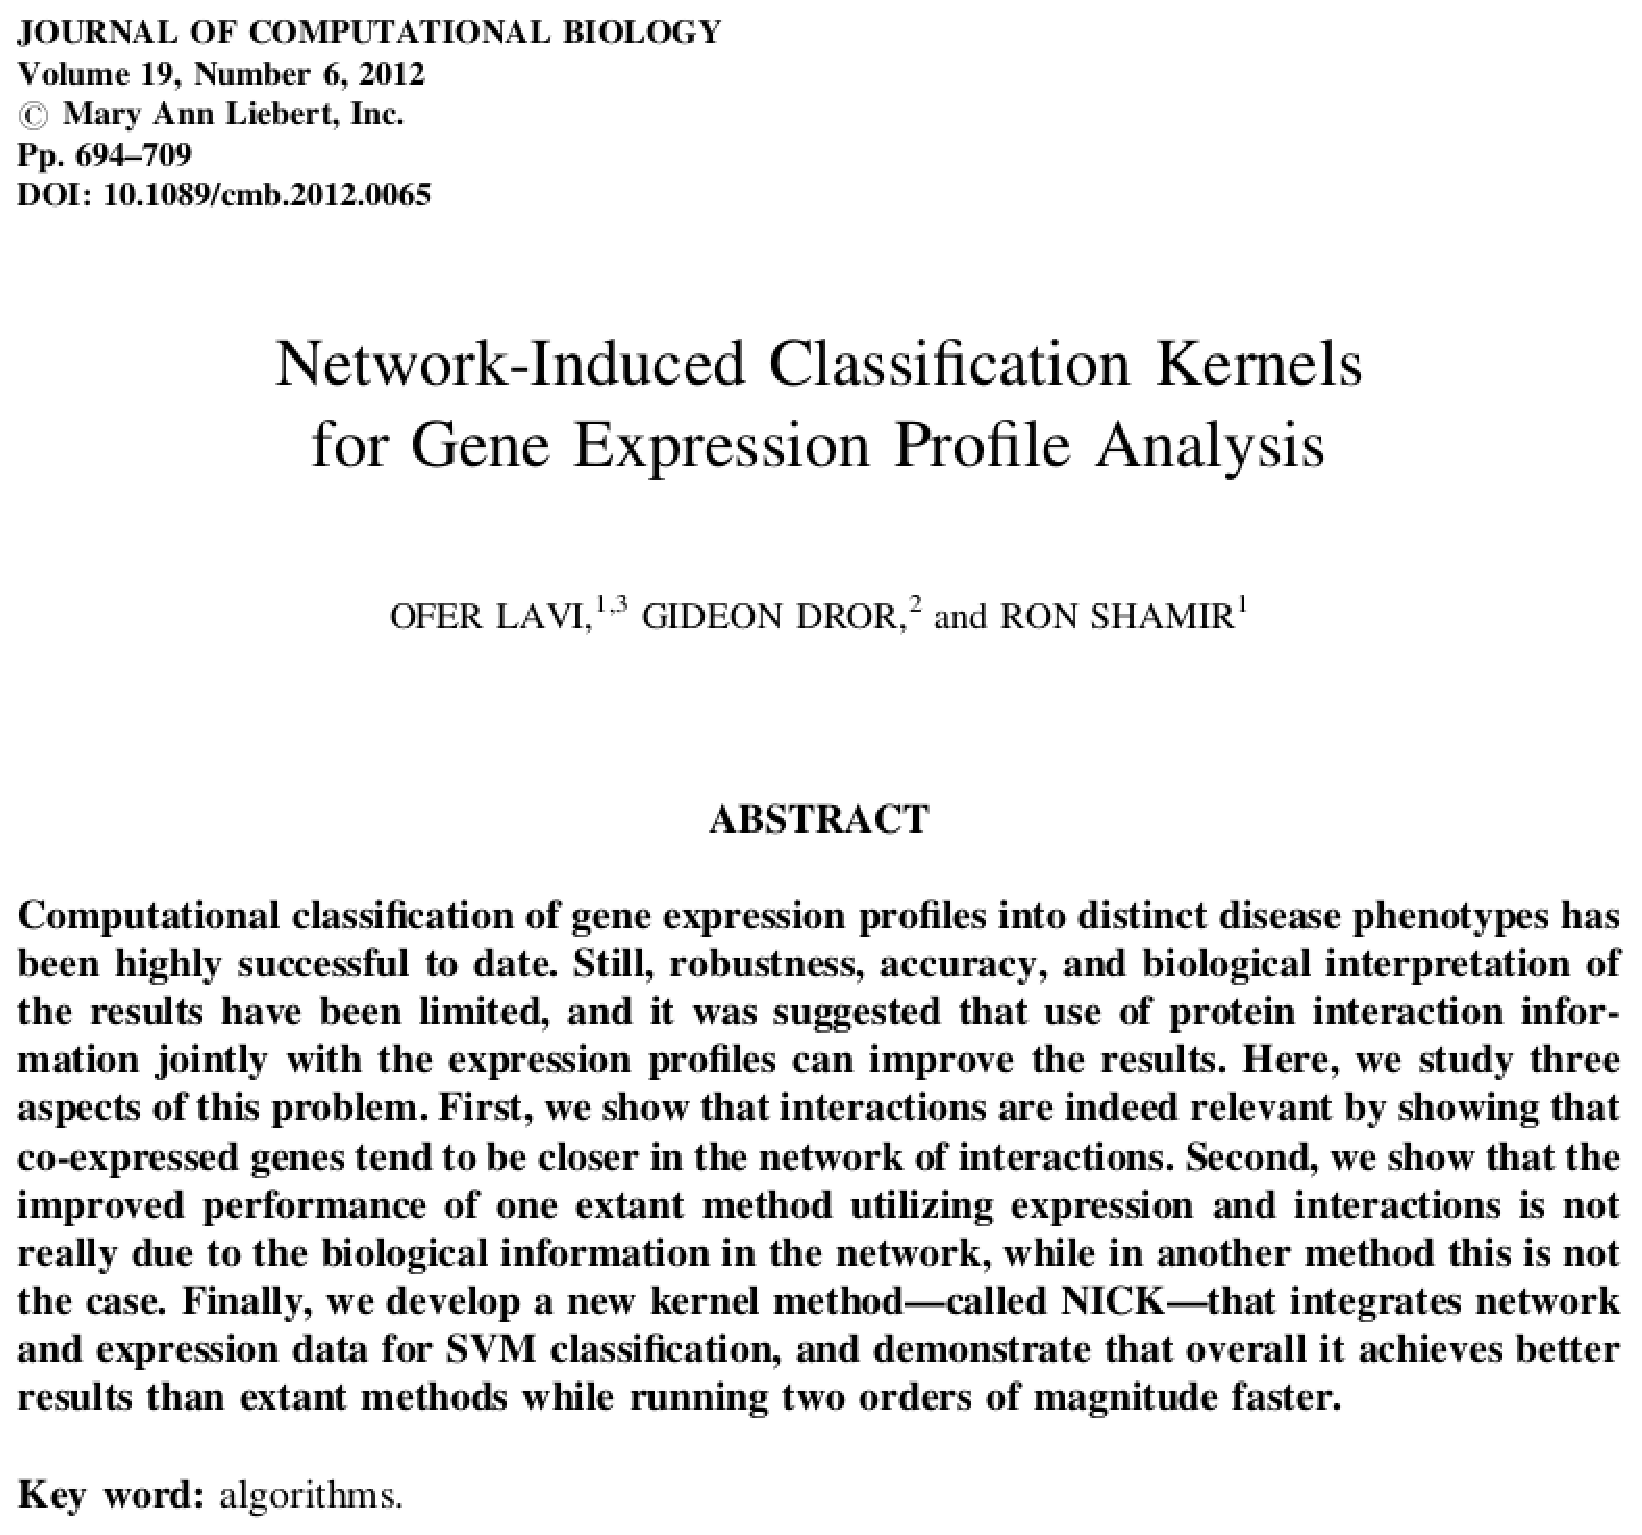
\includegraphics[width=1\textwidth]{NICK-paper}
            \end{figure}
          \end{column}
          \begin{column}{0.5\textwidth}
            \begin{enumerate}
            \item It's shown:
              \begin{itemize}
              \item Co-expressed genes tend to be close in the PPI-Network.
              \item Exploit this fact to modify the SVM objective function - called NICK
              \end{itemize}
            \item What can be done:
              \begin{itemize}
              \item Reverse engineer the learned machine to extract important genes after using the network information.
              \end{itemize}
            \end{enumerate}
          \end{column}
        \end{columns}
      \end{column}


      \begin{column}{0.3\textwidth}
        \begin{block}{NICK}
          \begin{columns}
            \begin{column}{0.5\textwidth}
              
              \begin{block}{\tiny{1. SVM modified objective function}}
                \tiny
                \begin{center}
                  $\min_{\mathbf{w}, w_0}\left\{\frac{1}{2}\|\mathbf{w}\|^2 + \frac{1}{2}\beta\sum_{(j,k)\in E}(w_j-w_k)^2\right\}$
                \end{center}
                s.t.:
                \begin{center}
                  $\forall i \in \{1,\cdots,n\} : (\mathbf{w}\mathbf{x}_i+w_0)y_i\geq 1$
                \end{center}
              \end{block}
              
              \begin{block}{\tiny{3. Dual to Primal}}
                \tiny
                \begin{center}
                  $\mathbf{w} = (\mathbf{I} + \beta \mathbf{B})^{-1} \sum_{i = 1}^n \alpha_i y_i \mathbf{x}_i$
                \end{center}
              \end{block}
            \end{column}
            
            \begin{column}{0.5\textwidth}
              \begin{block}{\tiny{2. Dual Problem}}
                \tiny
                \begin{center}
                  \begin{align*}
                    &\max_\alpha\left\{\sum_{i=1}^n\alpha_i-\frac{1}{2}\sum_{i=1}^n\sum_{j=1}^n\alpha_i\alpha_j y_i y_j (\mathbf{x}_i^T\mathbf{L})(\mathbf{L}^T\mathbf{x}_j)\right\}\\
                    &\mathbf{L}\mathbf{L}^T=(\mathbf{I}+\beta \mathbf{B})^{-1}\\
                    \text{s.t.: }&\\
                    &\forall i \in \{1,\cdots,n\}: \sum_{i=1}^n\alpha_iy_i=0\\
                    &\forall i \in \{1,\cdots,n\}: \alpha_i \geq 0 \\
                    &\text{Laplacian matrix:}\\  & \mathbf{B} = \mathbf{D} - \mathbf{A}
                  \end{align*}
                \end{center}
              \end{block}
            \end{column}
          \end{columns}
          %\mycite{Ofer Lavi, et.al., Journal of Computational Biology, (2012)}
        \end{block}
      \end{column}
    \end{columns}
  \end{block}

    %new row
    \begin{block}{Synthesize Data}
      \begin{columns}
        \begin{column}{0.3\textwidth}
          %\frametitle{Synthesize Data}
          \begin{enumerate}
          \item A random graph (PPI-Network)
          \item Signal nodes (genes): \[ f(n) = \left\{ 
            \begin{array}{l l}
              N(-\mu, 1) & \quad \text{if $n$ is in class $1$}\\
              N(\mu, 1) & \quad \text{if $n$ is in class $2$}
            \end{array} \right.\]
          \item Random nodes (non-informative genes): \[f(n) = N(0, 1) \]
          \item Pathway: 2, 3, or 4 connected signal nodes.
          \end{enumerate}
        \end{column}

        \begin{column}{0.3\textwidth}
          \begin{figure}
            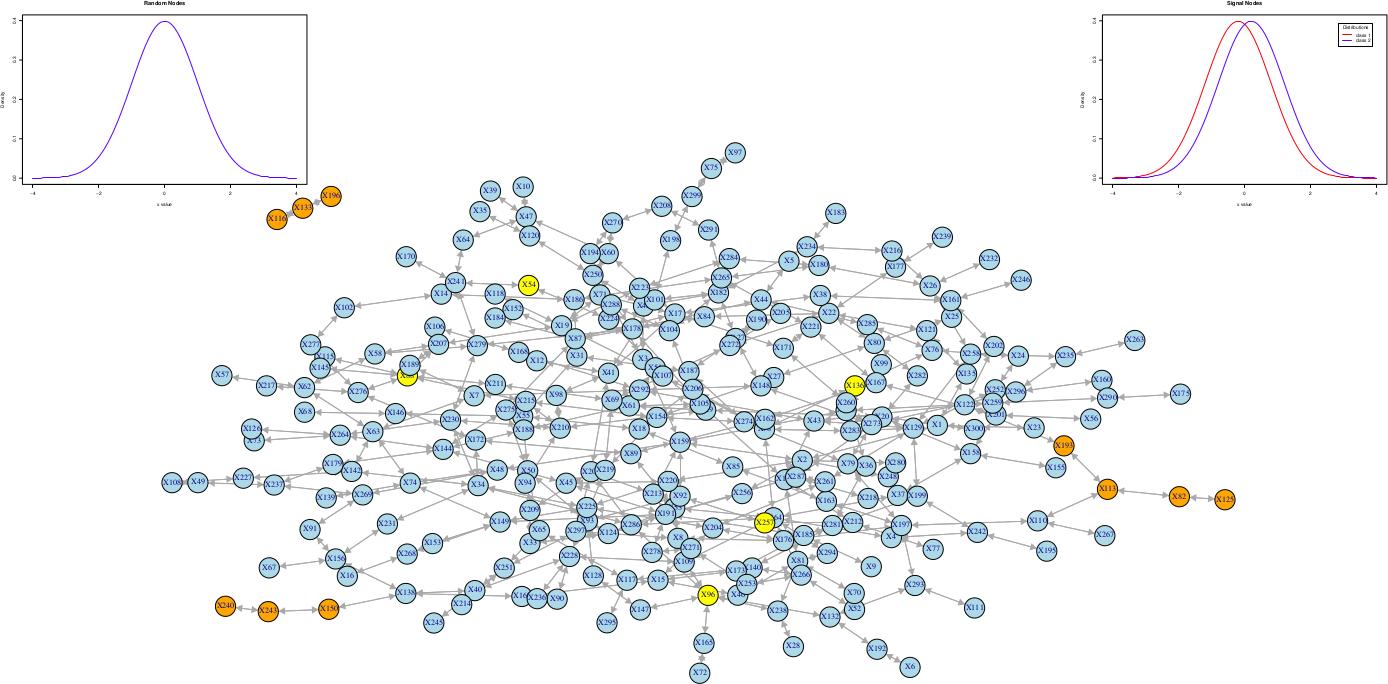
\includegraphics[width=0.8\textwidth]{synthesized-1slide}
            \caption{\tiny{{\color{blue}Blue}: random gene, {\color{orange}Orange}: Signal node being a member of a pathway of signal nodes, {\color{yellow}Yellow}: A lonely signal node}}
          \end{figure}
        \end{column}

        \begin{column}{0.3\textwidth}
          %\frametitle{Extract Important Genes}
          \begin{itemize}
          \item Solve SVM problem for original and transformed data.
          \item Calculate $\mathbf{w}$ for both models.
          \item Compute for each pair of nodes, for each model: 
            \begin{block}{}
              $Score(i, j) = \frac{|w_i| + |w_j|}{2} \times e^{max\left(d_G(i, j), 1\right)}$
            \end{block}
          \item Report pairs with highest scores for both trained models.
          \end{itemize}
        \end{column}
      \end{columns}
    \end{block}

    \begin{block}{Results}
      \begin{columns}
        \begin{column}{0.25\textwidth}
          %\frametitle{Synthesized Data Easy Scenario}
          \begin{figure}
            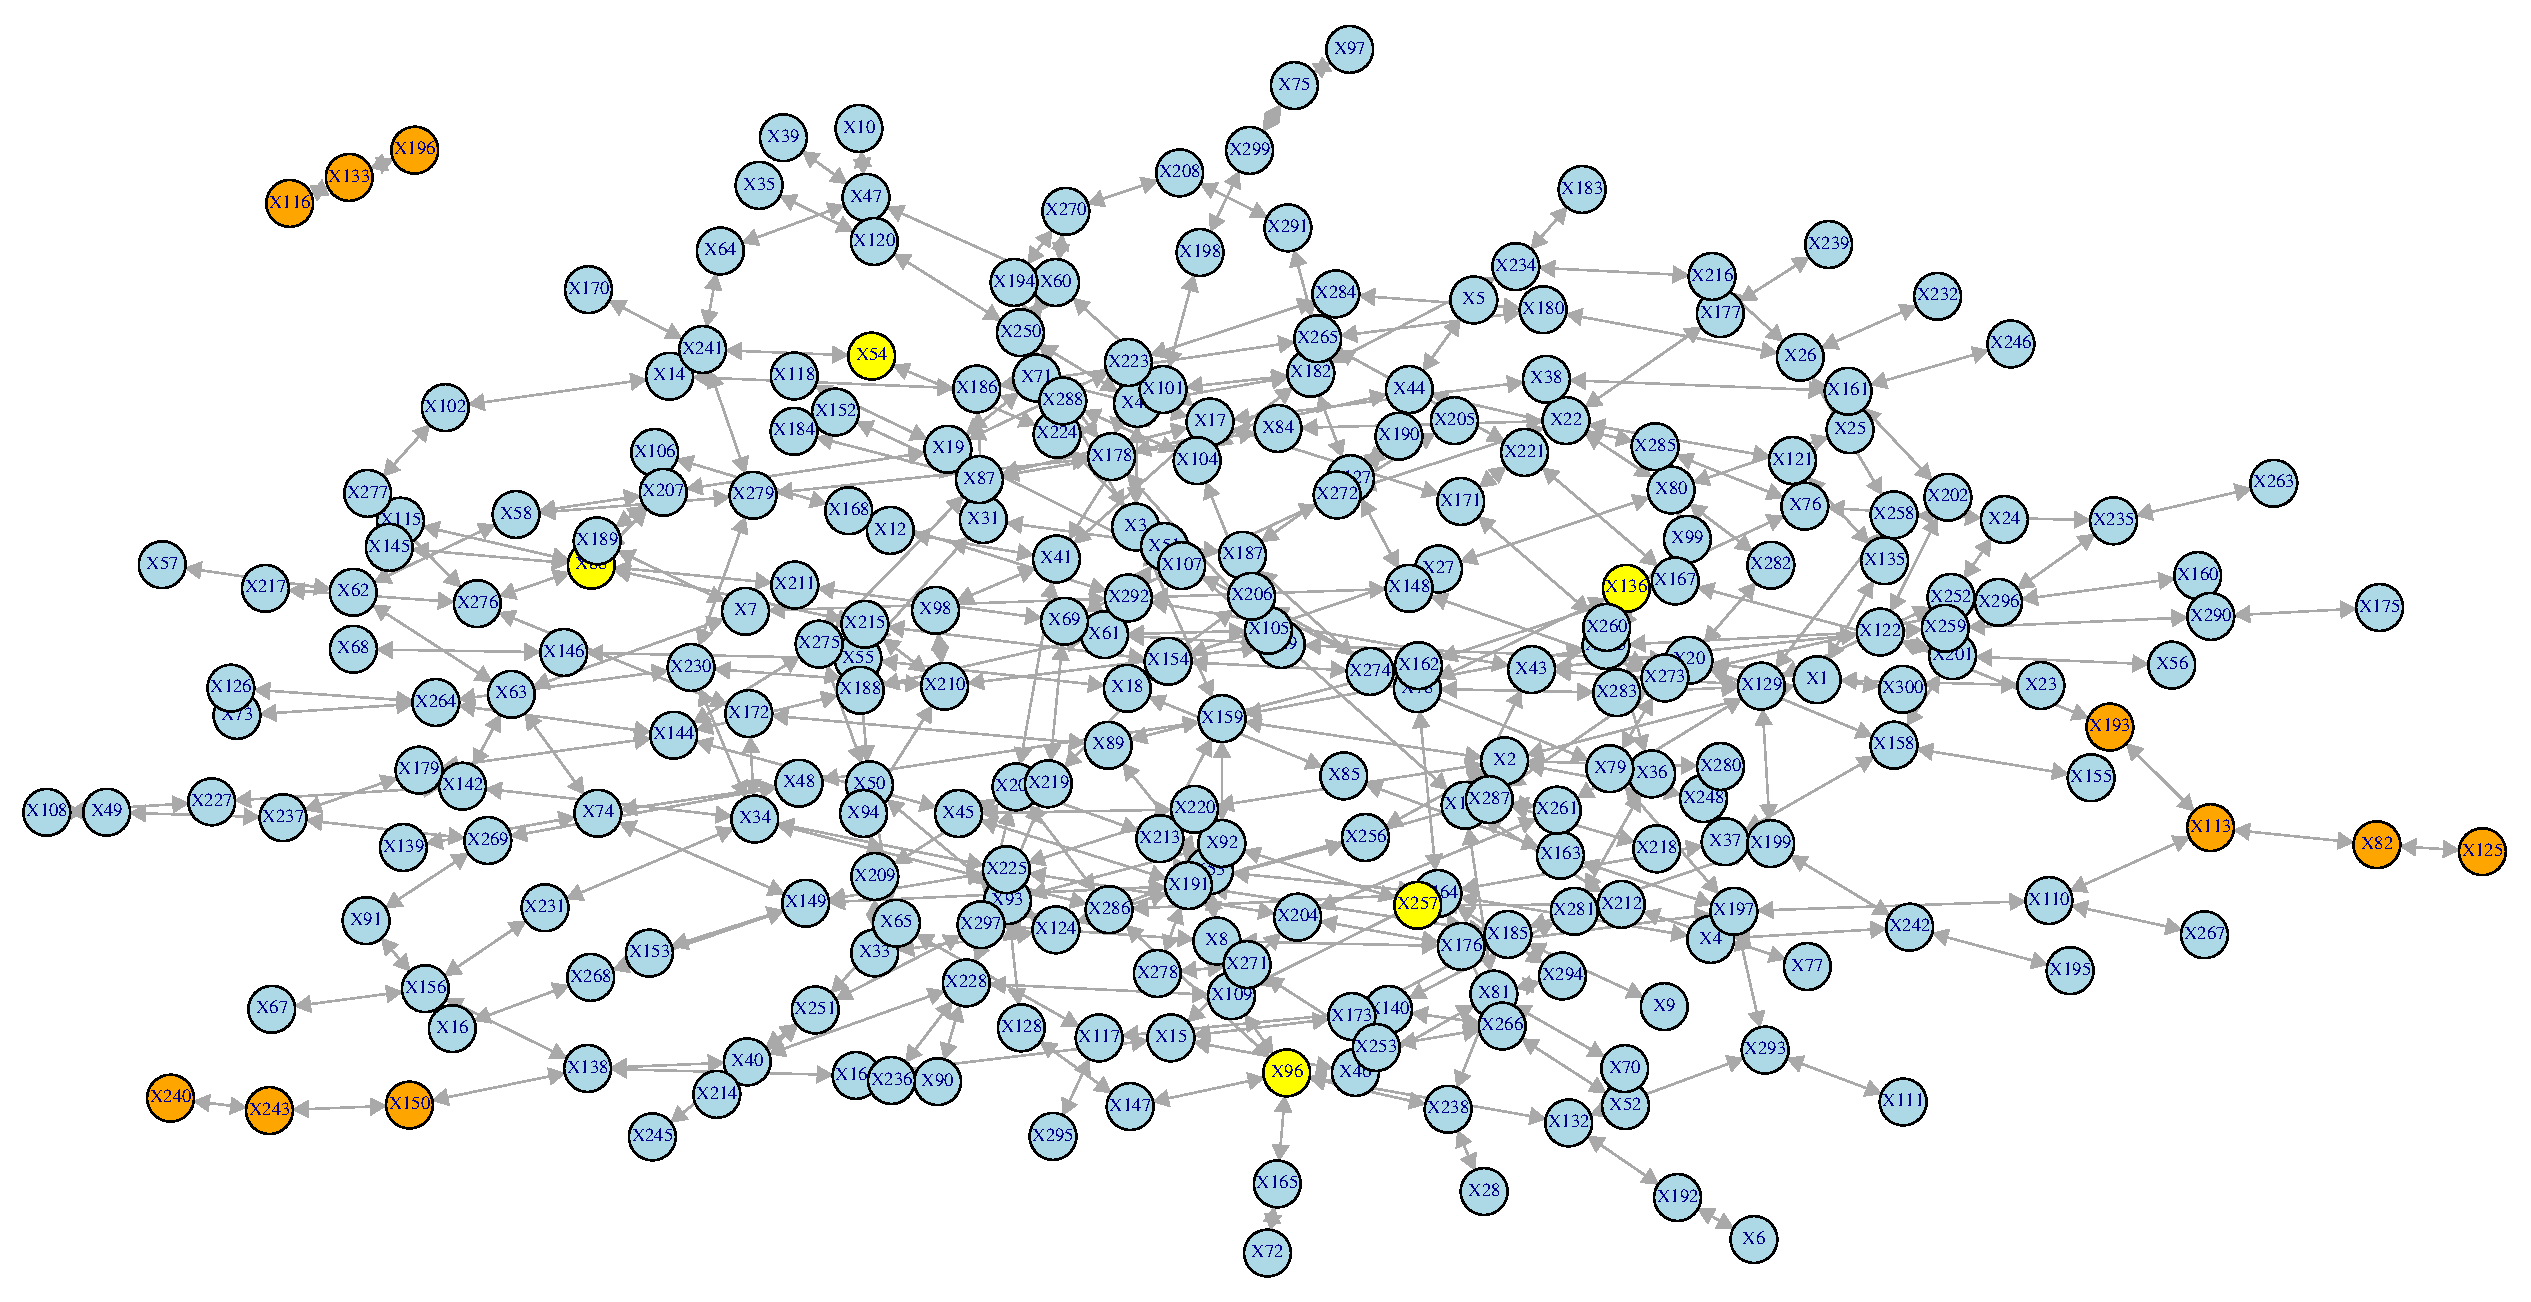
\includegraphics[width=\textwidth]{synthesized-easy}
            \caption{\tiny Easy}
          \end{figure}
          \begin{columns}
            \begin{column}{0.5\textwidth}
              \center
              \tiny
              \begin{tabular}{| c c || c c |}
                \hline
                \toprule
                \multicolumn{4}{c}{Original} \\ 
                \midrule \hline
                \boz X196   &  \boz X196  &
                X53   &  X53  \\ \hline
                X233   &  X233   &
                X39   &  X39  \\ \hline
                \ghool X88   &  \ghool X88  &
                \boz X196   &  \boz X133  \\ \hline
                \boz X116   &  \boz X116  &
                X127   &  X127  \\ \hline
                X197   &  X197  &
                X127   &  X148  \\ \hline
                X148   &  X148  &
                \boz X150   &  \boz X150  \\ \hline
                X148   &  X273  &
                \boz X116   &  \boz X133  \\ \hline
                X160   &  X160  &
                \ghool X96   &  \ghool X96  \\ \hline
                X95   &  X95  &
                X273   &  X273  \\ \hline
                \ghool X88   &  X115  &
                X40   &  X40  \\ \hline
                X53   &  X8  &
                X53   &  X164  \\ \hline
                X195   &  X195  &
                X56   &  X56  \\ \hline
              \end{tabular}
            \end{column}
            \begin{column}{0.5\textwidth}
              \center
              \tiny
              \begin{tabular}{| c c || c c |}
                \hline
                \toprule
                \multicolumn{4}{c}{Transformed} \\ 
                \midrule \hline
                \boz X196   &  \boz X196  &
                X233   &  X233  \\ \hline
                \boz X196   &  \boz X133  &
                \boz X133   &  \boz X133  \\ \hline
                \boz X133   &  \boz X116  &
                \boz X116   &  \boz X116  \\ \hline
                X95   &  X95  &
                \boz X240   &  \boz X240  \\ \hline
                X39   &  X39  &
                \boz X240   &  \boz X243  \\ \hline
                X59   &  X59  &
                X106   &  X106  \\ \hline
                \boz X243   &  \boz X243  &
                X106   &  X168  \\ \hline
                X114   &  X114  &
                X168   &  X168  \\ \hline
                \boz X243   &  \boz X150  &
                X56   &  X56  \\ \hline
                X39   &  X47  &
                X298   &  X298  \\ \hline
                \boz X150   &  \boz X150  &
                X247   &  X247  \\ \hline
                \boz X125   &  \boz X125  &
                X83   &  X83  \\ \hline
              \end{tabular}
            \end{column}
          \end{columns}
        \end{column}

        \begin{column}{0.25\textwidth}
          %\frametitle{Synthesized Data Medium Scenario}
          \begin{figure}
            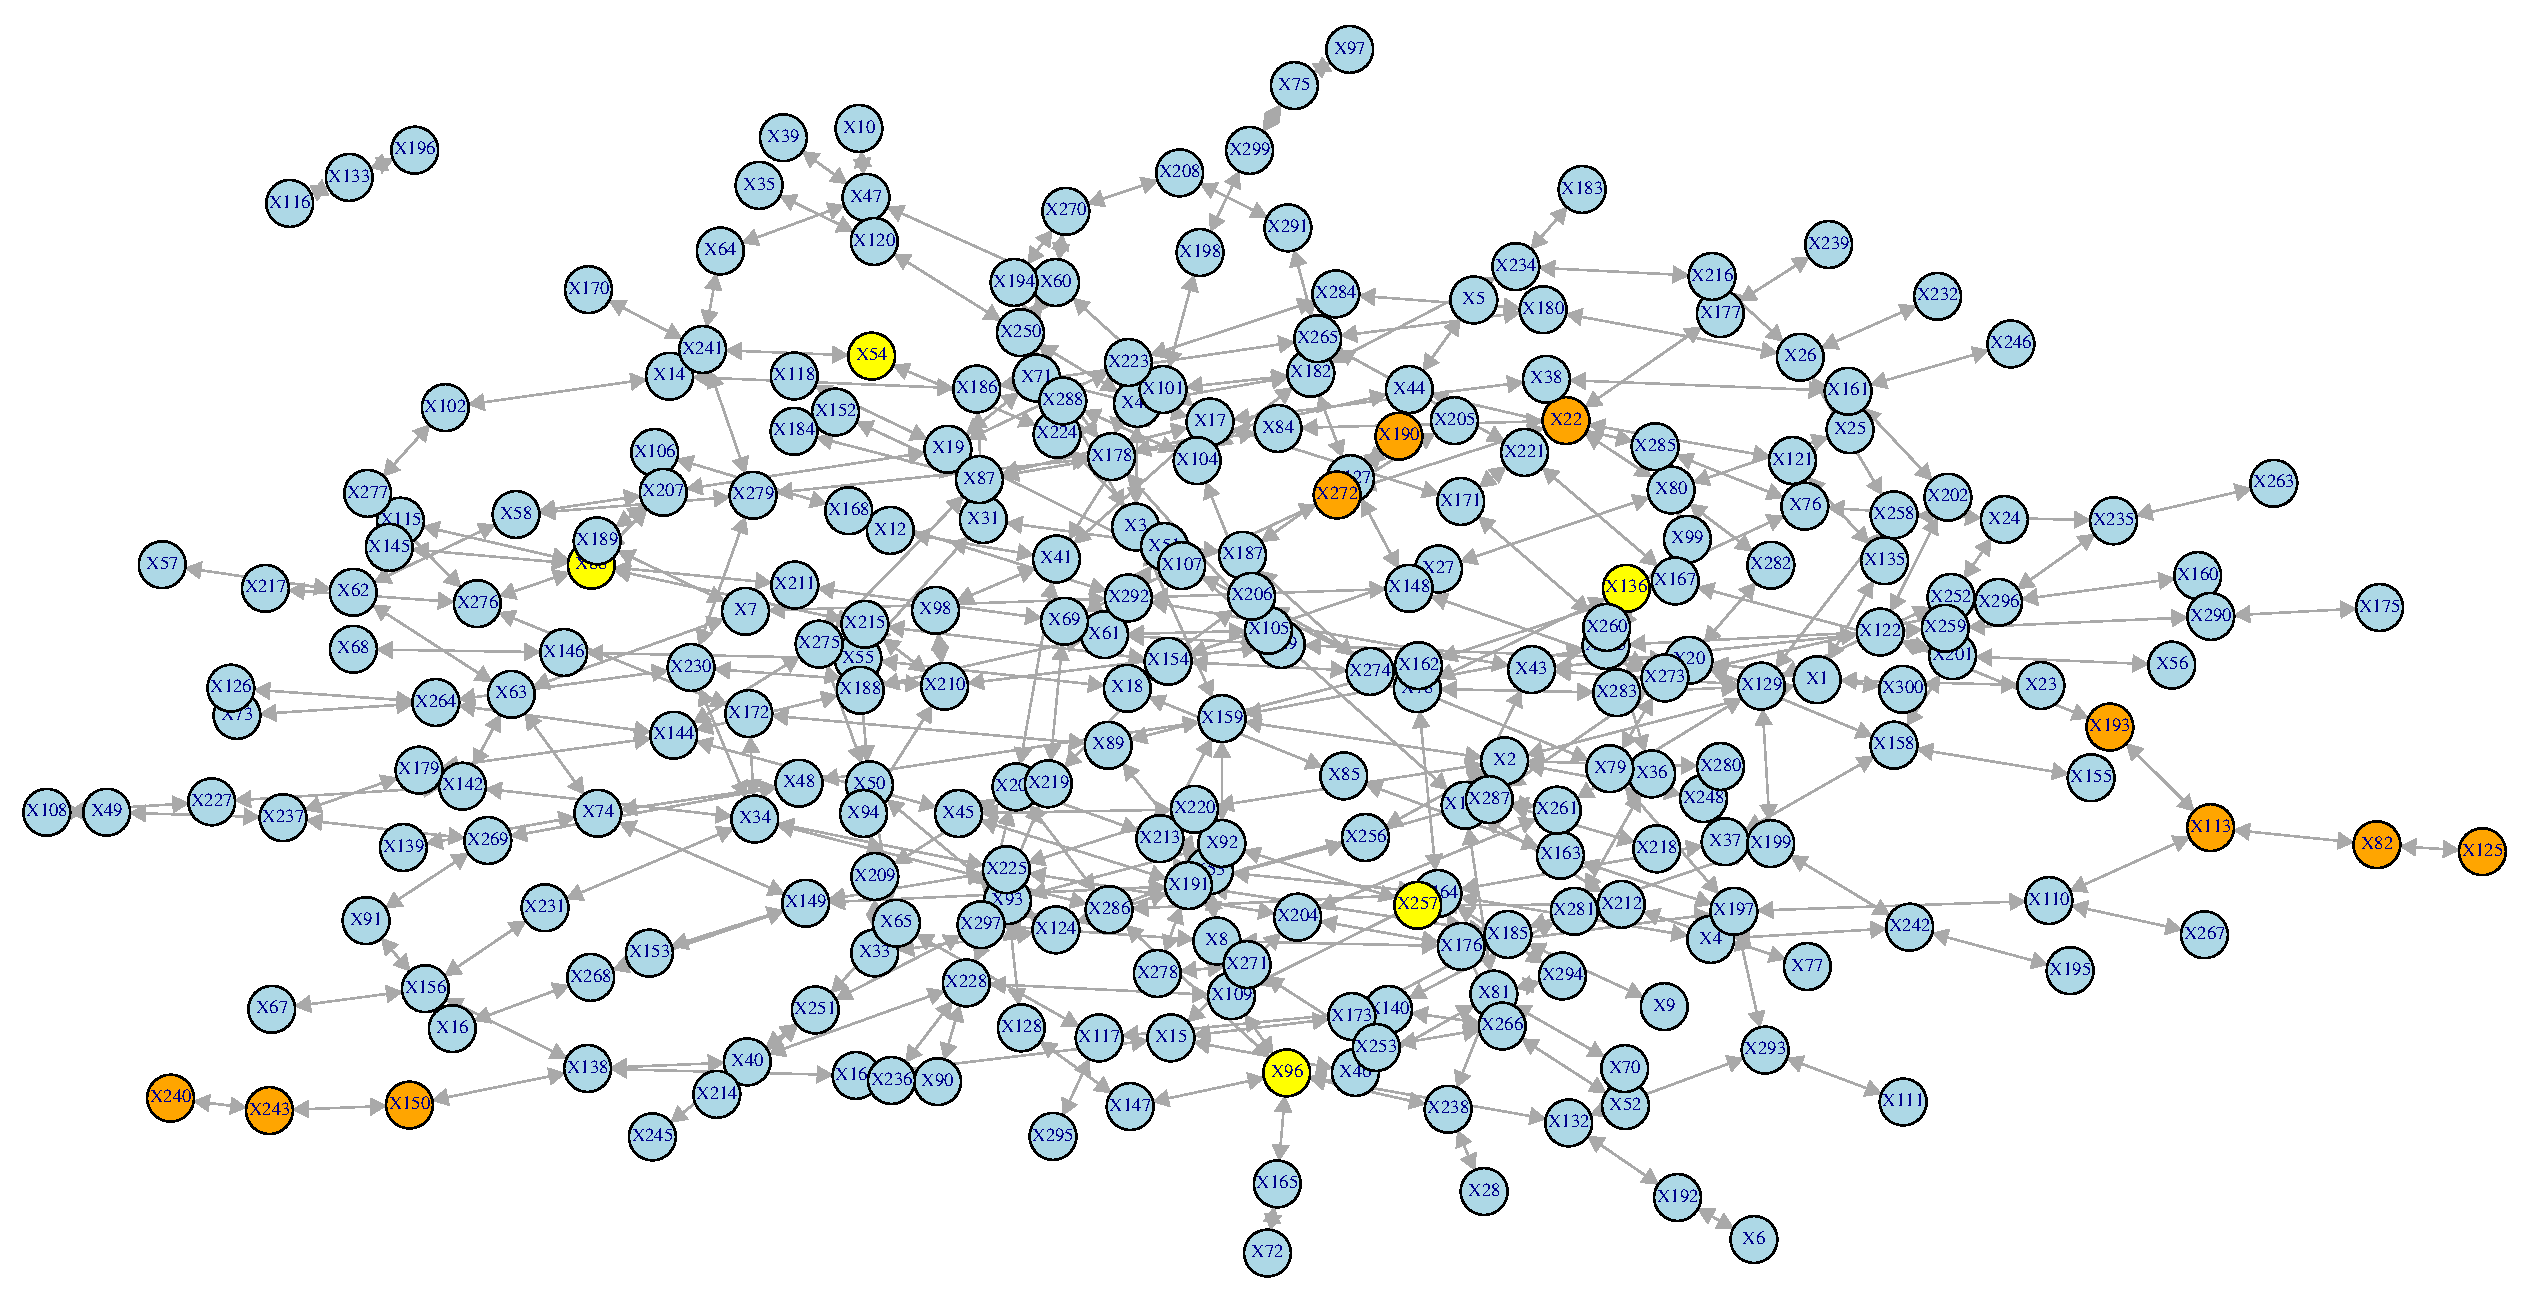
\includegraphics[width=\textwidth]{synthesized-medium}
            \caption{\tiny Medium}
          \end{figure}
          \begin{columns}
            \begin{column}{0.5\textwidth}
              \center
              \tiny
              \begin{tabular}{| c c || c c |}
                \hline
                \toprule
                \multicolumn{4}{c}{Original} \\ 
                \midrule \hline
                \boz X190   &  \boz X190 &
                X104   &  X104  \\ \hline
                X233   &  X233  &
                \boz X190   &  \boz X272  \\ \hline
                X277   &  X277  &
                \ghool X88   &  \ghool X88  \\ \hline
                \boz X190   &  X127  &
                X165   &  X165  \\ \hline
                \boz X272   &  \boz X272 &
                \boz X272   &  \boz X22  \\ \hline
                X106   &  X106  &
                X165   &  \ghool X96  \\ \hline
                \boz X150   &  \boz X150  &
                X250   &  X250  \\ \hline
                \ghool X88   &  X215  &
                \boz X22   &  \boz X22  \\ \hline
                X51   &  X51  &
                X28   &  X28  \\ \hline
                X73   &  X73  &
                X35   &  X35  \\ \hline
                X162   &  X162  &
                \boz X113   &  \boz X113  \\ \hline
                X112   &  X112  &
                X277   &  X102  \\ \hline
              \end{tabular}
            \end{column}
            \begin{column}{0.5\textwidth}
              \center
              \tiny
              \begin{tabular}{| c c || c c |}
                \hline
                \toprule
                \multicolumn{4}{c}{Transformed} \\ 
                \midrule \hline
                X233   &  X233  &
                \boz X190   &  \boz X190  \\ \hline
                X112   &  X112  &
                \boz X240   &  \boz X240  \\ \hline
                \boz X190   &  \boz X272 &
                \boz X240   &  \boz X243  \\ \hline
                X86   &  X86  &
                \boz X243   &  \boz X243  \\ \hline
                \boz X243   &  \boz X150 &
                \boz X190   &  X127  \\ \hline
                \boz X150   &  \boz X150  &
                \boz X272   &  \boz X272  \\ \hline
                X246   &  X246  &
                X298   &  X298  \\ \hline
                X106   &  X106  &
                \boz X125   &  \boz X125  \\ \hline
                X35   &  X35  &
                \boz X125   &  \boz X82  \\ \hline
                X247   &  X247  &
                \boz X272   &  X69  \\ \hline
                \boz X272   &  \boz X22 &
                \boz X82   &  \boz X82  \\ \hline
                X100   &  X100  &
                \ghool X257   &  \ghool X257  \\ \hline
              \end{tabular}
            \end{column}
          \end{columns}
        \end{column}

        \begin{column}{0.25\textwidth}
          \begin{figure}
            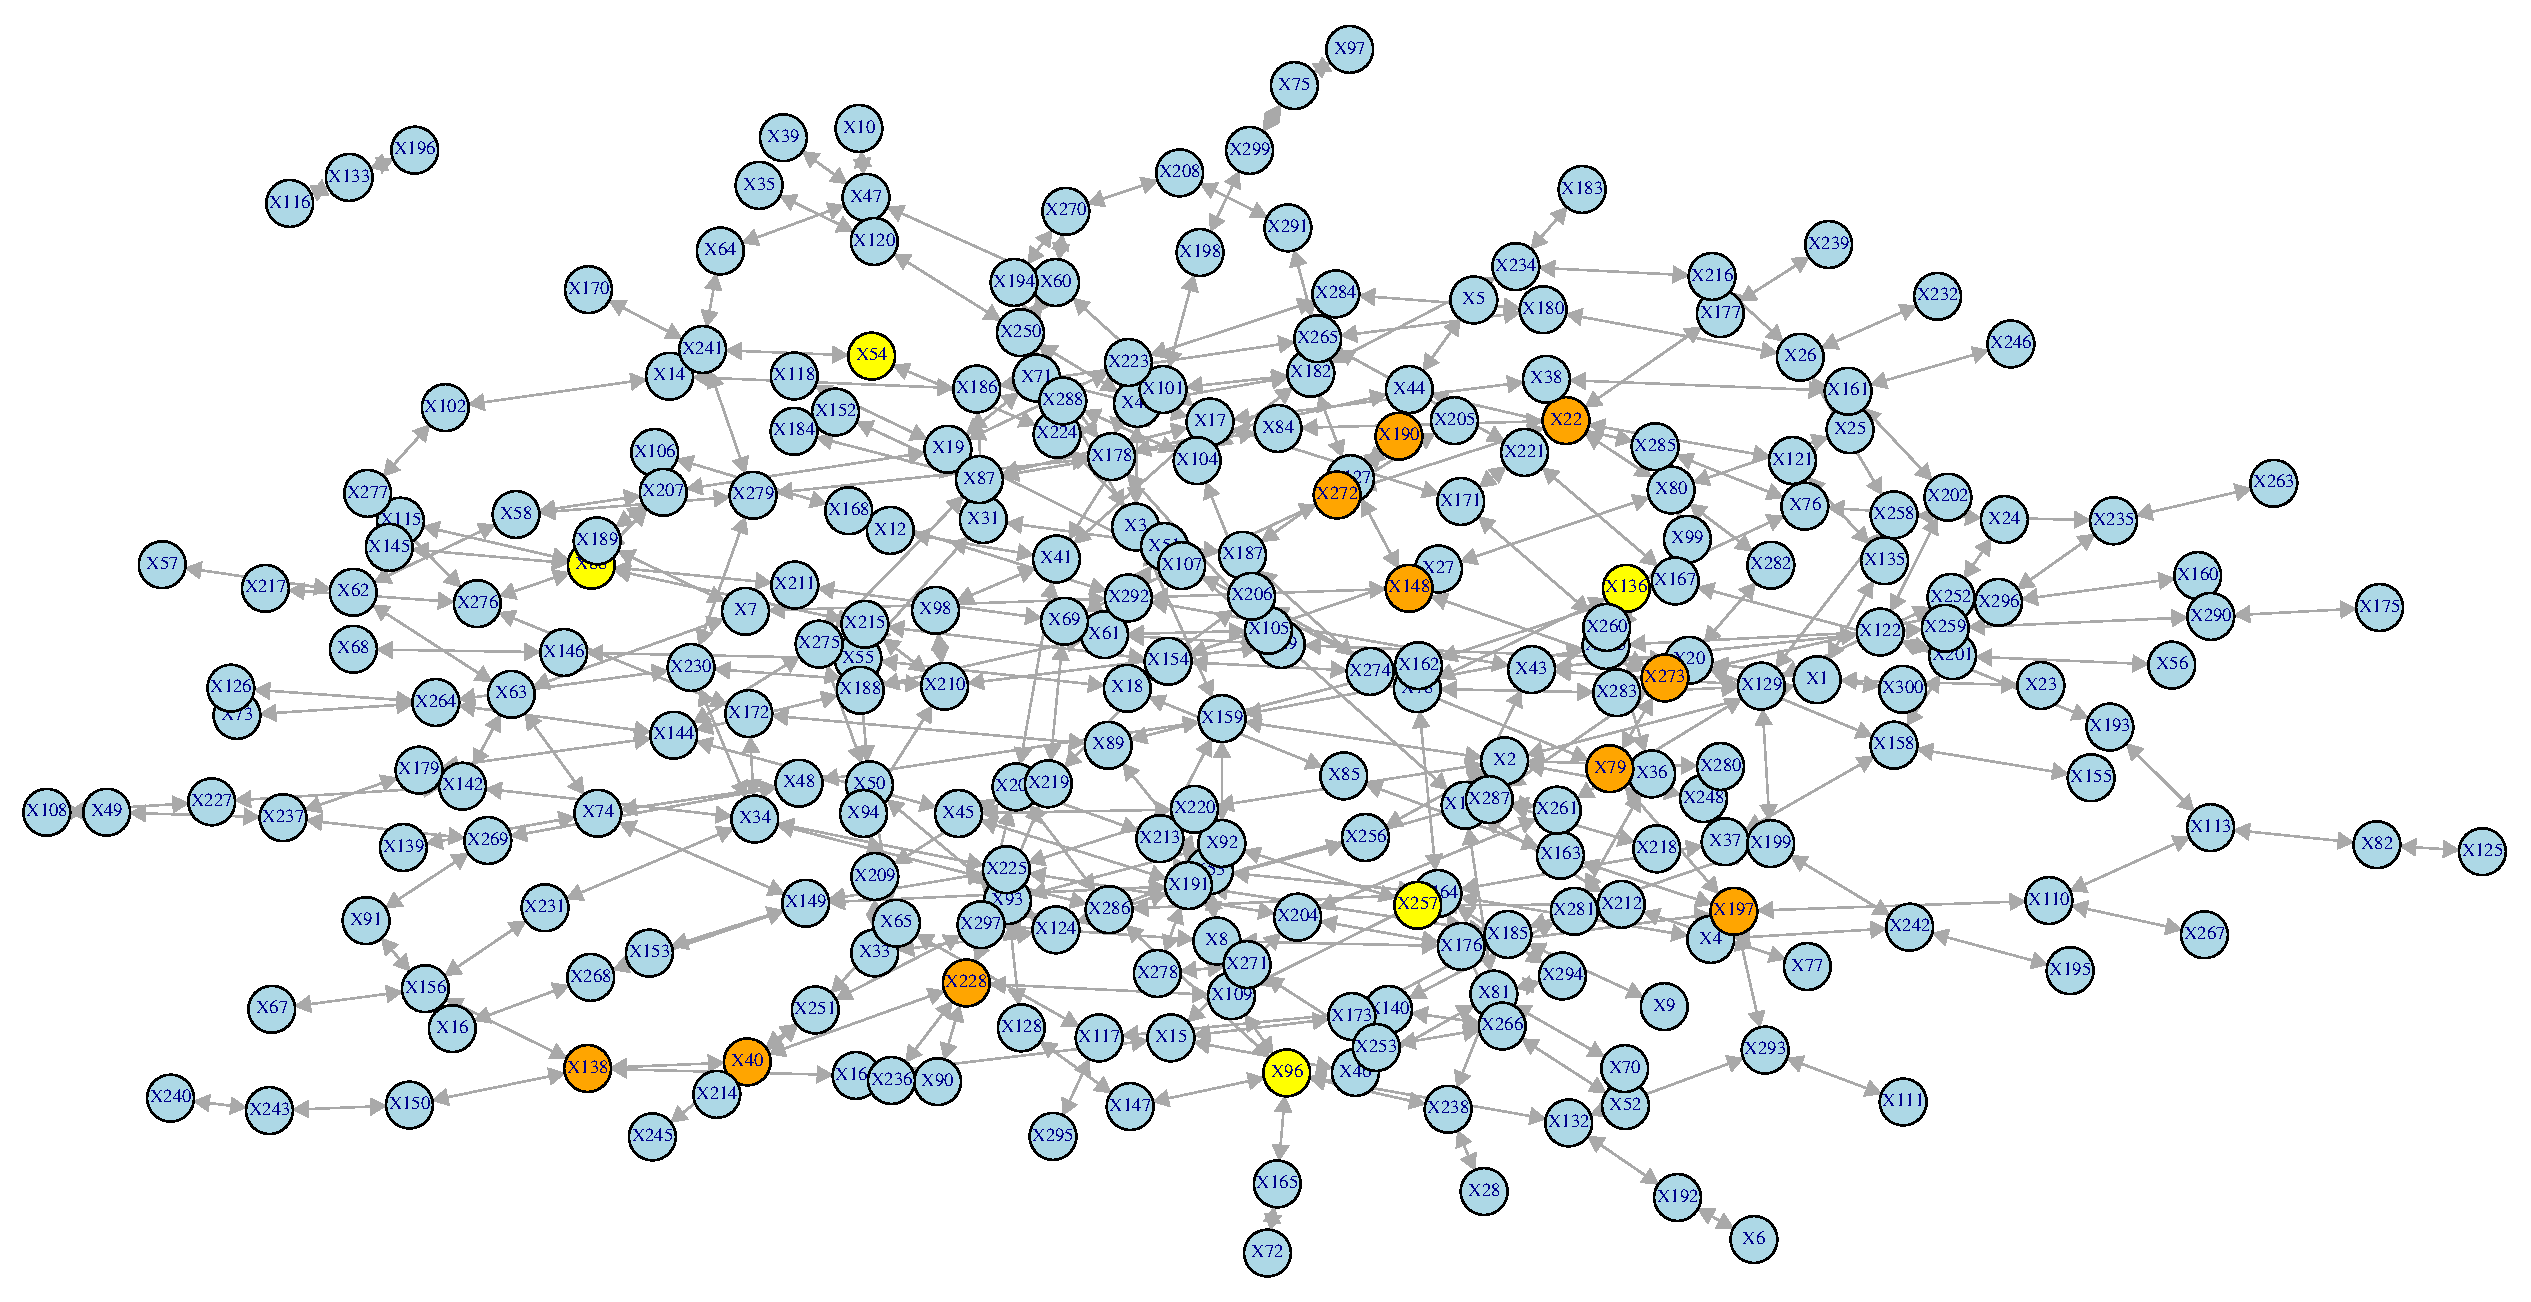
\includegraphics[width=\textwidth]{synthesized-hard}
            \caption{\tiny Hard}
          \end{figure}
          \begin{columns}
            \begin{column}{0.5\textwidth}
              \center
              \tiny
              \begin{tabular}{| c c || c c |}
                \hline
                \toprule
                \multicolumn{4}{c}{Original} \\ 
                \midrule \hline
                \boz X190   &  \boz X190  &
                X101   &  X101  \\ \hline
                X233   &  X233  &
                \boz X190   &  \boz X272  \\ \hline
                \ghool X88   &  \ghool X88  &
                X297   &  X297  \\ \hline
                \boz X190   &  X127  &
                X93   &  X93  \\ \hline
                X26   &  X26  &
                \boz X138   &  \boz X138  \\ \hline
                \boz X272   &  \boz X272 &
                \boz X272   &  \boz X22  \\ \hline
                X101   &  X41  &
                X123   &  X123  \\ \hline
                \boz X22   &  \boz X22 &
                X101   &  X198  \\ \hline
                X146   &  X146  &
                \boz X228   &  \boz X228  \\ \hline
                X278   &  X278  &
                X72   &  X72  \\ \hline
                \ghool X88   &  X115 &
                \ghool X96   &  \ghool X96  \\ \hline
                \boz X148   &  \boz X148 &
                X112   &  X112  \\ \hline
              \end{tabular}
            \end{column}
            \begin{column}{0.5\textwidth}
              \center
              \tiny
              \begin{tabular}{| c c || c c |}
                \hline
                \toprule
                \multicolumn{4}{c}{Transformed} \\ 
                \midrule \hline
                X233   &  X233  &
                \boz X190   &  \boz X190  \\ \hline
                X112   &  X112  &
                \boz X190   &  \boz X272  \\ \hline
                X86   &  X86  &
                \boz X190   &  X127  \\ \hline
                \boz X272   &  \boz X272 &
                \boz X272   &  X205  \\ \hline
                X205   &  X205  &
                X146   &  X146  \\ \hline
                X146   &  X68  &
                X68   &  X68  \\ \hline
                X298   &  X298  &
                \boz X272   &  \boz X22  \\ \hline
                X90   &  X90  &
                X127   &  X127  \\ \hline
                X100   &  X100  &
                \boz X272   &  X69  \\ \hline
                X297   &  X297  &
                X72   &  X72  \\ \hline
                X127   &  \boz X148 &
                X155   &  X155  \\ \hline
                X247   &  X247  &
                X196   &  X196  \\ \hline
              \end{tabular}
            \end{column}
          \end{columns}
        \end{column}

        \begin{column}{0.25\textwidth}
          \center
          \scriptsize
          \begin{tabular}{| c c |}
            \multicolumn{2}{c}{Easy} \\ 
            \midrule
            AUC (Original): & 60.6 \\ 
            AUC (Transformed): & 62.4 \\
            wc p-value (paired): & 5.669e-09 \\ 
            \toprule
            \multicolumn{2}{c}{Medium} \\ 
            \midrule
            AUC (Original): & 60.1 \\ 
            AUC (Transformed): & 61.5 \\ 
            wc p-value (paired): & 1.383e-06 \\ 
            \toprule
            \multicolumn{2}{c}{Hard} \\ 
            \midrule
            AUC (Original): & 60.6 \\ 
            AUC (Transformed): & 62.4 \\ 
            wc p-value (paired): & 5.669e-09 \\ \hline
          \end{tabular}        
        \end{column}
      \end{columns}
    \end{block}
  \end{frame}
\end{document}

